\section{Примеры}
\label{sec:samples}

\subsection{Простейшее уравнение эйконала}
\label{sec:simple-eikonal}

Рассмотрим несколько примеров и приложений для алгоритмов, описанных
выше. Для начала рассмотрим простой пример:


\begin{equation}
  \label{eq:eik-sur}
  \left\{ \begin{matrix}
      \| \nabla T(x) \| = 1, x \in \Omega \\
      T(x) = 0, x \in \Gamma
    \end{matrix}\right.
\end{equation}

В простейшем случае, мы считаем, что функция $F$ уравнение
\eqref{eq:eikonal} является константой и равна единице, т.е. после
дискретизации в каждой точке $\Omega$ функция $F$ принимает значение
$1$. Тогда решением будет концентрические окружности
рисунок~\ref{fig:eikonal-surface}, если же его рисовать в трехмерном
пространстве (см. Рисунок~\ref{fig:eikonal-surface-3d}).

\begin{figure}[H]
  \centering
  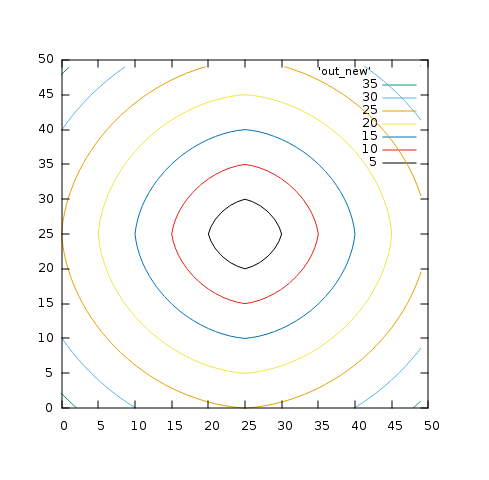
\includegraphics[width=\linewidth]{img/eikonal_simple_surface.png}
  \hfil \caption{Линии уровня численного решения эйконала с $F\equiv 1$ }
  \label{fig:eikonal-surface}
\end{figure}

\begin{figure}[H]
  \centering
  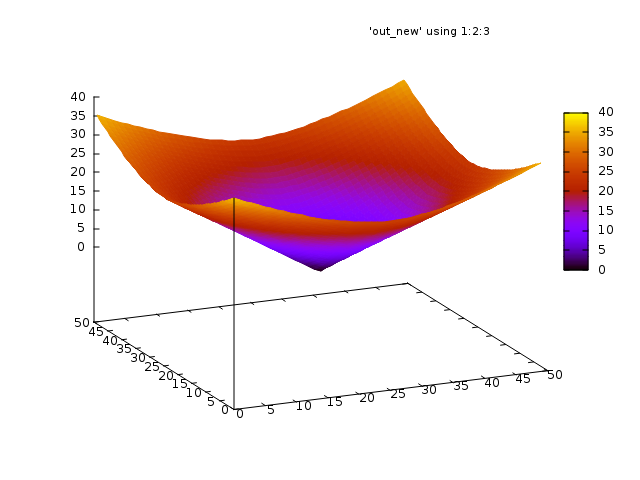
\includegraphics[width=\linewidth]{img/eikonal_simple_3d.png}
  \hfil \caption{Трехмерный график численного решения эйконала с $F\equiv 1$}
  \label{fig:eikonal-surface-3d}
\end{figure}

Если мы добавим барьер для распространения волн, т.е. в точках лежащих
на некотором прямоугольнике установим значение $0$. Мы получим
следующий результат. Смотри рисунок~\ref{fig:barier_surface}.

\begin{figure}[H]
  \centering
  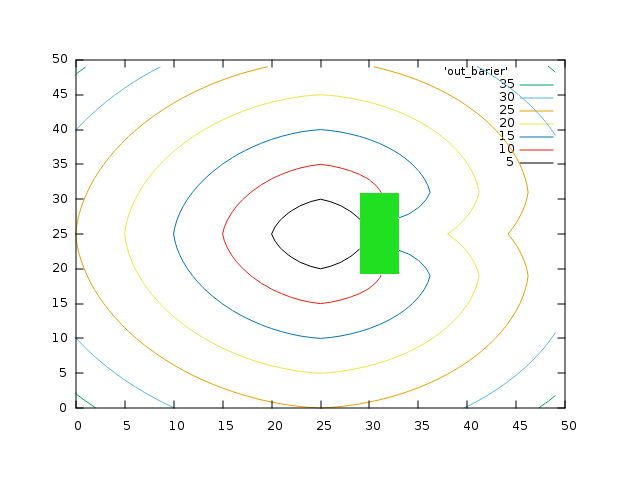
\includegraphics[width=\linewidth]{img/barier_surface.png}
  \hfil \caption{Линии уровня численного решения эйконала с $F\equiv
    1$, с препятствием}
  \label{fig:barier_surface}
\end{figure}

\subsection{Множество достижимости импульсной системы}
\label{sec:ids}

В работах \cite{AVS2016, AV2015_1,AV2015_2} предлагалось считать
множество достижимости импульсной управляемой системы. В
использованном в тех работах методе были существенные ограничения на
систему ограничений на управление, а именно в том, что для описаний
ограничений на управлении использовалась $l_1$ метрика. Методы
численных решений уравнений эйконала позволяют нам использовать
евклидову метрику, правда за счет некоторого упрощения самих уравнений

Для начала взглянем на обычную управляемую систему, расширение
множества траекторий которой и приводит к импульсной системе. Будем
работать с системой следующего вида. 

\begin{equation}
  \label{system_s}
  \begin{array}{l}
    \dot{x}(t)=E \cdot F(x)v(t), \quad x(0)=x_0, \\[8pt]
    v(t)\geq 0  \qquad \forall\, t\in T = [0,t_1], \qquad
    \displaystyle\int_{0}^{t_1} ||v(t)||dt\leq V.
  \end{array} 
\end{equation}

Здесь
\begin{itemize}
  \item $E$ --- единичная матрица.
  \item $||v||:=\sqrt{v_1^2+v_2^2}$
  \item $x(\cdot)$ --- абсолютно непрерывная вектор-функция
    (траектория), $x(t)\in {\mathbb R}^n,$
  \item $v(\cdot)$ --- измеримая существенно ограниченная
    вектор-функция (управление),
  
  \item $V$ --- заданная величина интегрального ресурса управления
    $v$.
\end{itemize}

Пару функций $\bigl(x(\cdot),v(\cdot)\bigr),$ удовлетворяющих
системе \eqref{system_s}, будем называть процессом системы \eqref{system_s}.

Будем предполагать, что вектор-функция $f$ является функцией из
$L_{\infty}(T,\mathbb{R}^2)$.
     
Множество обычных траекторий системы \eqref{system_s} будет состоять
из функций, имеющих равномерно ограниченные полные вариации на отрезке
$T$. Следовательно, любая последовательность траекторий будет
содержать подпоследовательность, поточечно сходящуюся к некоторой
функции ограниченной вариации. Именно такие функции, являющиеся
поточечными пределами последовательностей обычных траекторий, в
дальнейшем будут называться разрывными (или обобщенными) решениями
системы \eqref{system_s}.

 Рассмотрим систему \eqref{system_d} соответствующую системе
\eqref{system_s}.

\begin{equation}
  \label{system_d}
  \begin{array}{l}
    dx(t)=f\big(t,x(t)\big)dt+G\big(t,x(t)\big)\pi(\mu), \quad
    x(0)=x_0, \\[8pt]
    \pi(\mu) \in \mathcal{W}(T)
  \end{array} 
\end{equation}

Здесь $T=[0,t_1]$ --- заданный отрезок времени, $x(\cdot)$ ---
непрерывная справа на $(0,t_1]$ функция ограниченной вариации, $x(t)
\in \mathbb{R}^2$. Решения системы \eqref{system_d}, соответсвующие
управлению $\pi(\mu)$, понимаются как решения интегрального уравнения
с мерой
\begin{equation*}
  x(t) = x_0  + \int_0^t E\cdot F(t,x(t)) \mu_c(dt) +
  \sum_{s \le t,\\s \in S_d(\mu)} (z_s(d_s) - x(s-)), \quad t \in (0,t_1]
\end{equation*}
где для каждого $s \in S_d(\mu)$ функция $z_s(\cdot)$ --- решение
дифференциального уравнения
\begin{equation*}
  \frac{dz_s(\tau)}{d\tau} = E\cdot f(s,z_s(\tau))\omega_s(\tau), \quad z_s(0)=x(s-)
\end{equation*}

Таким образом, при расширении системы \eqref{system_s} и переходе к
соответствующей импульсной системе \eqref{system_d} мы к обычным
(абсолютно непрерывным) траекториям добавляем все частичные
поточечные пределы последовательностей обычных
траекторий. Полученное множество будем называть множеством
траекторий импульсной системы, соответствующей \eqref{system_s} и будем
обозначать импульсную систему символом \eqref{system_d} Поясним,
что если в системе \eqref{system_d} траектории могут иметь скачки,
то их обобщенные производные будут содержать дельтообразные
составляющие --- импульсы; следовательно, импульсы появятся в
соответствующих управлениях, отсюда и названия импульсной системы и
импульсного управления.


Функция ограниченной вариации $x(\cdot)$ называется траекторией
импульсной системы \eqref{system_d} (или обобщенным (разрывным)
решением системы \eqref{system_s}), если найдется такая последовательность
траекторий системы \eqref{system_s} $\bigl\{x_k(\cdot)\bigr\}$, что выполняется
условие 
\begin{equation*}
  x_k(t)\to x(t) \quad  \forall \, t\in [0,T].
\end{equation*}

Определим \emph{множество достижимости} в момент  времени $t=t_1$
импульсной системы \eqref{system_d}. Обозначим это множество через 
$ {\mathcal R}_V(t_1)$. Это множество из  пространства ${\mathbb R}^n$
(конечномерное  множество), оно состоит из точек $x_b,$ в  которые в
момент $t=t_1$ попадают траектории  системы \eqref{system_d}, выходящие
в начальный  момент из начальной точки $x_0$.

Возьмем пример динамической системы:

\begin{equation*}
  \begin{aligned}[b]
    &\dot{x_1}(t) = (1/((x_1(t)+0.1) * (x_2(t)+0.1))v_1(t), & x_1(0)=50\\
    &\dot{x_2}(t) = (1/((x_1(t)+0.1) * (x_2(t)+0.1))v_2(t), & x_2(0) = 50\\[8pt]
    &v_1(t) \ge 0, v_2(t) \ge 0 \\
    &\int_{0}^{1} \sqrt{(v_1(t)^2) + (v_2(t))^2} dt \le V
  \end{aligned}
\end{equation*}

Множеством достижимости для конкретного $V$ здесь будут все значения
решения, которые меньше или равны заданному $V$. Численные методы
решения эйконала порождают интегральную воронку: все возможные
множества достижимости для значения $V \in [0,V_{max}]$

На рисунке~\ref{fig:impulse-example-levels} представлено такая
интегральная воронка через линии уровня.

\begin{figure}[H]
  \centering
  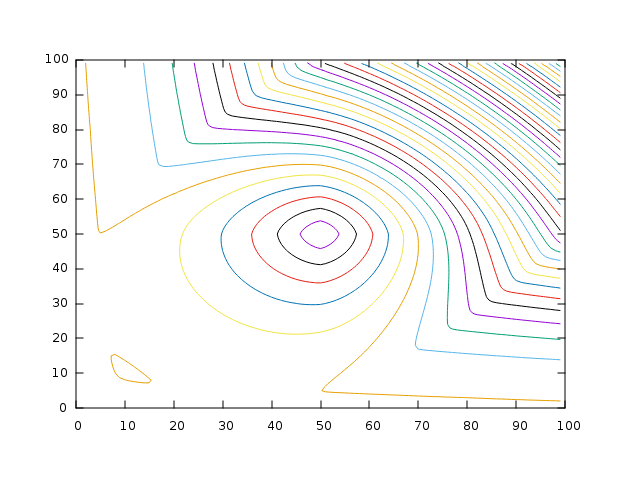
\includegraphics[width=\linewidth]{img/impulse-example-levels.png}
  \hfil \caption{Линии уровня множества достижимости}
  \label{fig:impulse-example-levels}
\end{figure}

В виде трехмерной поверхности график можно увидеть на рисунке~\ref{fig:impulse-example}

\begin{figure}[H]
  \centering
  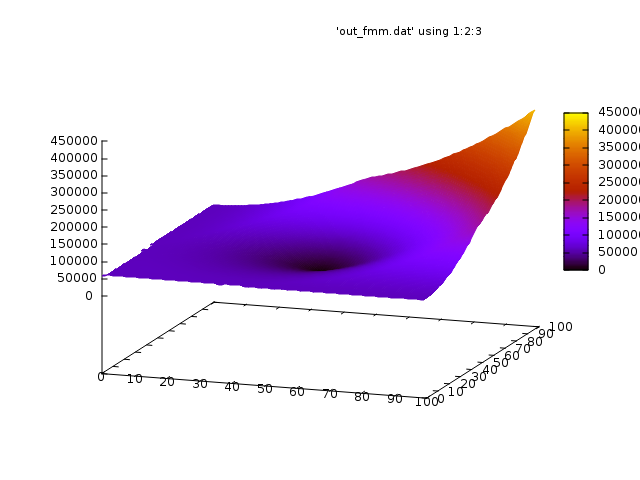
\includegraphics[width=\linewidth]{img/impulse-example.png}
  \hfil \caption{Интегральная воронка в трехмерном виде}
  \label{fig:impulse-example}
\end{figure}


\subsection{Shape from shading}
\label{sec:shape-from-shading}

Еще одним важным приложением численных алгоритмов решения уравнения
эйконала является задача восстановления по черно-белой картинке (или
фотографии) форму исходного объекта \cite{SFS2009}. Это понятие также
не переводится в русскоязычных публикациях. Дословно это понятие
значит построение поверхности от тени. На изображении, лишенном цвета,
нашему глазу предоставляется информация о яркости соответствующей
точки. Наш глаз может благодаря ей строить форму объекта.  

Яркость изображения пропорциональна излучению от поверхности к
наблюдателю

\begin{equation}
  \label{eq:sfs:1}
  E_i=\mu L_s,
\end{equation}

где параметр $\mu$ зависит от параметров камеры (таких как диаметр
линзы, фокальное расстояние и т.д.).
Мы полагаем, что источник освещения один и находится примерно там же,
где и глаз наблюдателя. Кроме того отсутствуют отражения. Яркость
изображения пропорциональна излучению поверхности, изображенной на
нем. В этом случае отношение между излучением точки поверхности с
нормалью в этой точке и направлением к источнику света описывается 
Двулучевой функцией отражательной способности (ДФОС), которая является
константой для Ламбертиановской поверхности.

\begin{equation}
  \label{eq:sfs:4}
  L_s=\frac{\alpha}{\pi}E_s,
\end{equation}
где $\alpha$ --- альбедо, а $E_s$ --- интенсивностью
излучения. Наконец, интенсивность излучения $E_s$ определяется как:

\begin{equation}
  \label{eq:sfs:5}
  E_s = I_0\frac{cos(\theta_i)}{r^2},
\end{equation}
где $I_0$ это интенсивность источника света, $r$ --- расстояние между
источником света и точкой поверхности и $theta_i$ --- угол между
нормалью к точке поверхности и направлением на источник света.

Из \eqref{eq:sfs:1}, \eqref{eq:sfs:4} и \eqref{eq:sfs:5} получим яркость
изображения:

\begin{equation}
  \label{eq:sfs:6}
  E_i = \sigma\frac{cos(\theta_i)}{r^2},
\end{equation}
где $\sigma$ это постоянный коэффициент, связанный с параметрами
системы формирования изображения, интенсивности источника света и
альбедо поверхности.


На языке python был написан скрипт (листинг 8), который переводит информацию по
яркости изображения в параметр искривления поверхности, т.е. чем выше
яркость, тем меньше в этой точке наклон поверхности относительно
ортогонального к нам. Тем самым мы получаем $F$ для уравнения
эйконала, по которой ищем решение. Оно и будет той самой поверхностью,
которую нам нужно достать из фотографии

\vspace{1em}
Листинг 8 --- Скрипт преобразования яркости изображения в 
\normalsize
\begin{verbatim}
#!/usr/bin/env python

from PIL import Image
import scipy as sc
import sys
import math

def main():
    im = Image.open(sys.argv[1])
    print im.height* im.width, 3
    data = sc.asarray(im.convert("L"))

    out = sc.empty([im.height, im.width])

    max_out = 0
    
    max_val = data.max()
    lst = []
    for i in range(len(data)):
        for j in range(len(data[i])):
            if abs(data[i][j]) > 0.01:
                tst = math.sqrt((1.0*max_val/data[i][j])**2 - 1)
                if abs(tst) > 0.1:
                    out[i][j] = 1.0/tst
                else:
                    out[i][j]= sc.inf
            else:
                out[i][j]= 0
            if out[i][j]>max_out:
                max_out = out[i][j]

    for i in range(len(data)):
        for j in range(len(data[i])):
            if data[i][j]==max_val:
                print i,j,out[i][j],0
            else:
                print i,j,out[i][j],sc.inf

if __name__ == '__main__':
    main()
\end{verbatim}
\large

    

%%% Local Variables:
%%% mode: latex
%%% TeX-master: "eikonal_solver"
%%% End:
